\subsection{Velocity Field for a Rigid Body}


\begin{frame}{Introduction}
\begin{figure}[ht]
	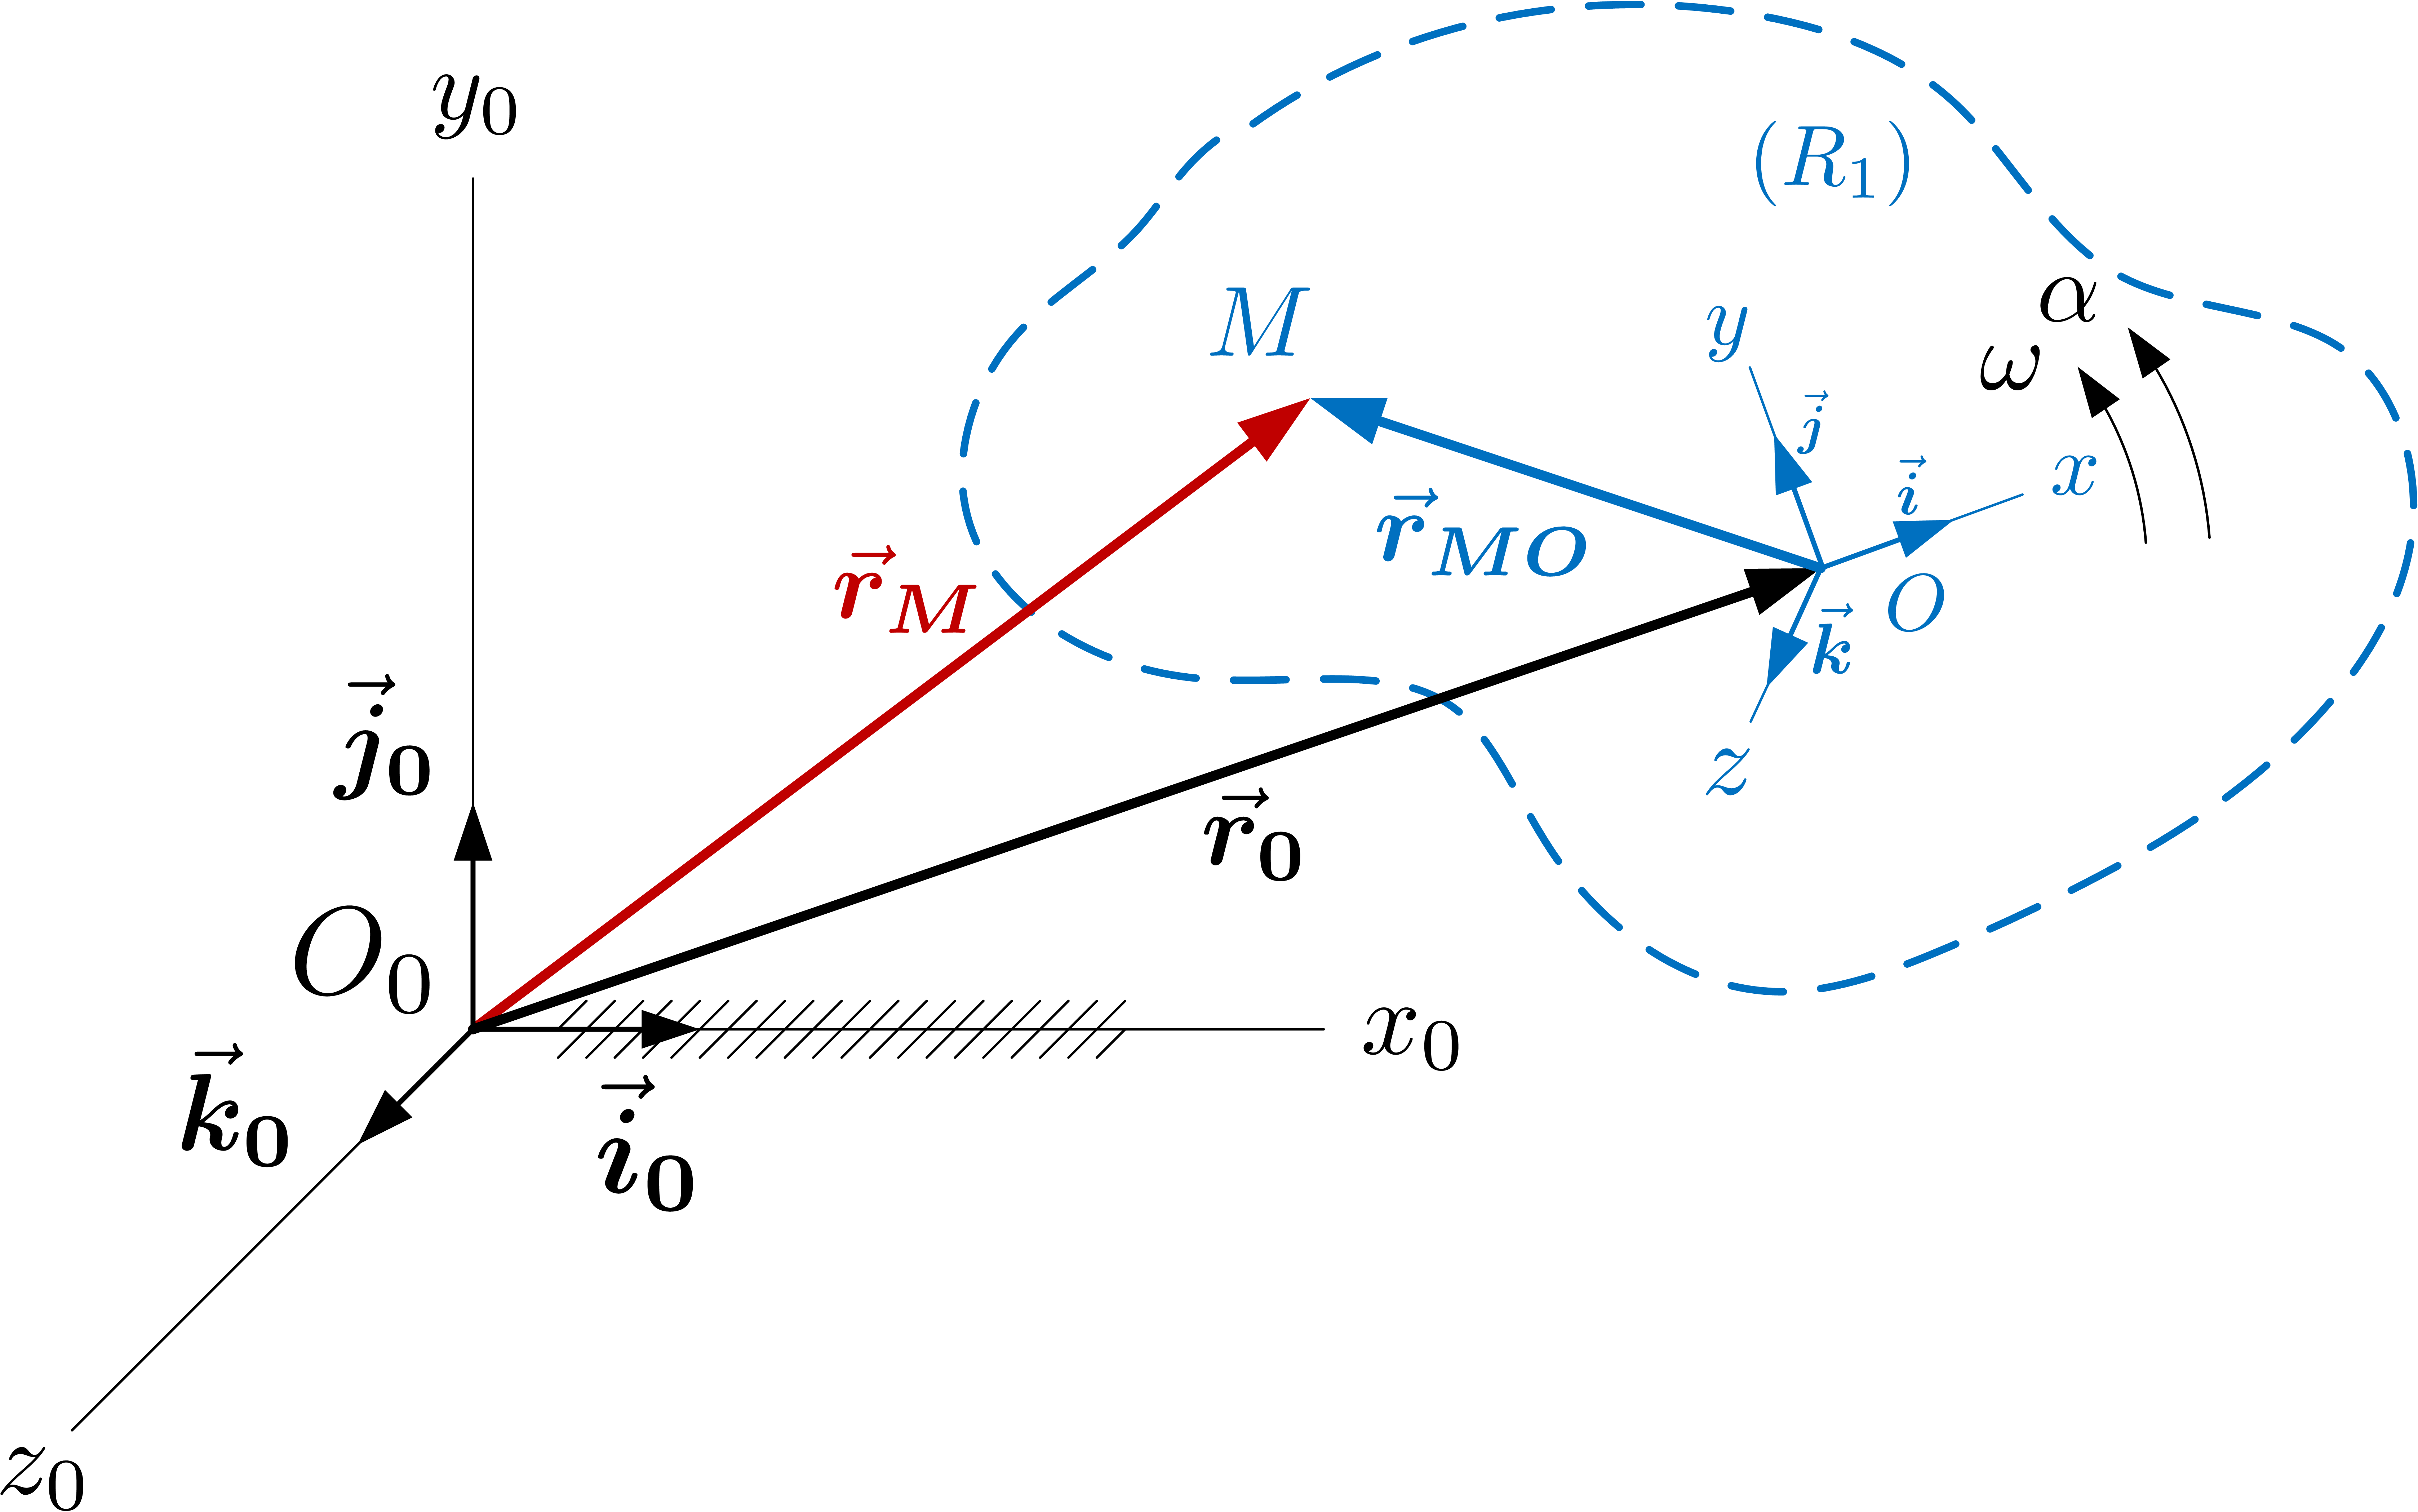
\includegraphics[width=80mm]{images/v_a.png}
\end{figure}
	Let $M$ be a point in rigid body $(R_1)$. Then $\vb{r}{M}$ is the position vector of $M$ relative to fixed reference frame $(O_0x_0y_0z_0)$.
	\[
	\vb{r}{M} = \vb{r}{O} + \vb{r}{MO} = \vb{r}{O} + x\ih+y\jh+z\kh
	\]
\end{frame}

\begin{frame}
	For Cartesian coordinates, the following relations are true:
	\[\begin{cases}
		\ih\cdot\ih=\jh\cdot\jh=\kh\cdot\kh=1\\
		\ih\cdot\jh=\jh\cdot\kh=\kh\cdot\ih=0
	\end{cases}\]
	
	Velocity vector $\vb{v}{M}=\xvec[.]{\bm{r}}_{\bm{M}}$ with respect to time $t$:
	\[
	\vb{v}{M} = \vb{v}{O} + \dot{x}\ih + \dot{y}\jh + \dot{z}\kh + x\frac{d\ih}{dt} + y\frac{d\jh}{dt} + z\frac{d\kh}{dt}
	\]
	
	For a rigid body, $\dot{x}=\dot{y}=\dot{z}=0$
	\[
	\Rightarrow\vb{v}{M}=\vb{v}{O}+x\frac{d\ih}{dt}+y\frac{d\jh}{dt}+z\frac{d\kh}{dt}
	\]
\end{frame}

\begin{frame}
	Let $\vb{\omega}{} = \omega_x\ih + \omega_y\jh + \omega_z\kh$ be rotational vector of rigid body $(R_1)$. Then
	\[
	\vb{\omega}{} = (\frac{d\ih}{dt}\cdot\jh)\ih+ (\frac{d\jh}{dt}\cdot\kh)\jh + (\frac{d\kh}{dt}\cdot\ih)\kh\]\[\hskip 13mm=(-\ih\cdot\frac{d\jh}{dt})\ih+(-\jh\cdot\frac{d\kh}{dt})\jh+(-\kh\cdot\frac{d\ih}{dt})\kh
	\]
	Combine with the fact that $\displaystyle \frac{d\ih}{dt}\cdot\ih=\frac{d\jh}{dt}\cdot\jh=\frac{d\kh}{dt}\cdot\kh=0$\vskip1.25mm
	$\displaystyle \frac{d\ih}{dt}=(\frac{d\ih}{dt}\cdot\ih)\ih + (\frac{d\ih}{dt}\cdot\jh)\jh + (\frac{d\ih}{dt}\cdot\kh)\kh= 0\ih+\omega_z\jh-\omega_y\kh=\vb{\omega}\times\ih$\\
	$\displaystyle \frac{d\jh}{dt}=(\frac{d\jh}{dt}\cdot\ih)\ih + (\frac{d\jh}{dt}\cdot\jh)\jh + (\frac{d\jh}{dt}\cdot\kh)\kh=-\omega_z\ih+0\jh+\omega_x\kh=\vb{\omega}\times\jh$\\
	$\displaystyle \frac{d\kh}{dt}=(\frac{d\kh}{dt}\cdot\ih)\ih + (\frac{d\kh}{dt}\cdot\jh)\jh + (\frac{d\kh}{dt}\cdot\kh)\kh= \omega_y\ih-\omega_x\jh+0\kh=\vb{\omega}\times\kh$
	\[
	\Rightarrow\vb{v}{}=\vb{v}{O}+\vb{\omega}{}\times(x\ih+y\jh+z\kh)
	\]
\end{frame}

\begin{frame}
	\begin{block}{Formula}
		For any point of a rigid body, its velocity equation is:
		\[
		\vb{v}{} = \vb{v}{O} + \vb{\omega}{}\times\vb{r}{}
		\]
		where $\vb{\omega}{}\times \vb{r}{}$ is the rotational motion of that point with respect to $O$
	
	\end{block}
	\emph{Example}\vskip 2.5mm
	In matrix form, velocity vector $\vb{v}{M}$ of point $M$ relative to fixed reference frame $(O_0x_0y_0z_0)$ can be written as:
	\[
	\vb{v}{M}=
	\begin{bmatrix}
	v_x\\v_y\\v_z
	\end{bmatrix}=
	\begin{bmatrix}
	v_{Ox}+z\omega_y-y\omega_z\\v_{Oy}+x\omega_z-z\omega_x\\v_{Oz}+y\omega_x-x\omega_y
	\end{bmatrix}=
	\vb{v}{O}+\vb{\omega}{}\times\vb{r}{MO}
	\]
\end{frame}